% This is samplepaper.tex, a sample chapter demonstrating the
% LLNCS macro package for Springer Computer Science proceedings;
% Version 2.20 of 2017/10/04
%
\documentclass[runningheads]{llncs}
%------------------------------------------------------------------------------------- (LIBRARIIES)
\usepackage{graphicx}
\usepackage{listings}
\usepackage{color}
\usepackage{hyperref}
% to display URLs in blue roman font according to Springer's eBook style:
\renewcommand\UrlFont{\color{blue}\rmfamily}
\usepackage{subfigure}
\usepackage{minted}


%------------------------------------------------------------------------------------- (LIBRARIIES-END)


% Default fixed font does not support bold face
\DeclareFixedFont{\ttb}{T1}{txtt}{bx}{n}{12} % for bold
\DeclareFixedFont{\ttm}{T1}{txtt}{m}{n}{12}  % for normal

% Custom colors
\definecolor{deepblue}{rgb}{0,0,0.5}
\definecolor{deepred}{rgb}{0.6,0,0}
\definecolor{lessdeepred}{rgb}{0.3,0,0}
\definecolor{deepgreen}{rgb}{0,0.5,0}


%------------------------------------------------------------------------------------- (DO NOT DELETE)
% Python style for highlighting
\newcommand\pythonstyle{\lstset{
language        =Python,
basicstyle      =\fontsize{7}\ttm,
morekeywords    ={self},              % Add keywords here
keywordstyle    =\fontsize{7}\ttb\color{deepblue},
emph            ={MyClass,FeatureExtractor,__init__, None, True},        % Custom highlighting
emphstyle       =\fontsize{7}\ttb\color{deepred},    % Custom highlighting style
stringstyle=\color{deepgreen},
frame=tb,                         % Any extra options here
showstringspaces=false
}}

% Python environment
\lstnewenvironment{python}[1][]
{
\pythonstyle
\lstset{#1}
}
{}

% Python for external files
\newcommand\pythonexternal[2][]{{
\pythonstyle
\lstinputlisting[#1]{#2}}}

% Python for inline
\newcommand\pythoninline[1]{{\pythonstyle\lstinline!#1!}}
%------------------------------------------------------------------------------------- (DO NOT DELETE-ENDE)






%------------------------------------------------------------------------------------- (Dokument)
\begin{document}

\title{Digital Libraries - Document Fingerprints}

%------------------------------------------------------------------------------------- (Title)
\author{Richard Hohensinner\inst{1}\orcidID{00273237} \and \\
Inti Gabriel Mendoza Estrada\inst{1}\orcidID{11804156} \and     \\
Jürgen Suntinger-Schrampf\inst{1}\orcidID{00630894}}

\authorrunning{R. Hohensinner et al.}
% First names are abbreviated in the running head.
% If there are more than two authors, 'et al.' is used.
\institute{TU Graz, Austria \\ GROUP 11}
\maketitle              % typeset the header of the contribution
%------------------------------------------------------------------------------------- (Title-ENDE)

%------------------------------------------------------------------------------------- (Abstract)
\begin{abstract}
The human is the best pattern recognition system on the whole world and has no problems when it comes to detecting outliers or finding patterns in a visual way. However, when it comes to textual data, the human brain has problems detecting or recognizing such things in an efficient way. At this point the computer comes into play, which extracts a sum of so called features (characteristics), which can then visualized just the way the human prefers it most, Visually. In our case, that happened over heatmaps which should help the user to do a vizual analysis under the help of interactive tools to find the so called literal-\textbf{fingerprints} (characteristic) of an author.

\end{abstract}
\keywords{Document fingerprint  \and Digital libraries \and Visualisation}
%------------------------------------------------------------------------------------- (Abstract-ENDE)


XXXXXXXX
%------------------------------------------------------------------------------------- (Introduction)
\section{Introduction}
As the world enters an era defined by \textit{big data}, more and more information is being actively accrued. This vast amount of data is not immediately available to people. It must now be accessible. What libraries did for physical books, digital libraries are doing for digital data. Challenges begin to appear when you consider that data can come in a vast array of ways (on top of the actual amount of data). When challenges appear, however, their solutions end up, most often than not, incredibly useful. Digital libraries not only let you access texts, papers, books. You are able to access videos, images, 3D models\ldots What makes digital libraries so incredibly useful lies in the fields it comprises: Computer Science, Information Science, and Information Visualisation - to name a few. 

In Computer Science comes something called \textit{Natural Language Processing} (or NLP). NLP is the automatic understanding of text by a computer. Being able to "understand" text is immensely useful. In the field of Digital Libraries, therefore, you can not only access text via keywords or titles but also through what the text actually means and compels.

What if you could search through a text based on the emotions of sentences? What if you could find texts that are easy to read based on sentence length? What if you could find texts to improve your language skills based on sentence complexity? What if you could use NLP to train a Neural Network to guess the genre of a text? This is the motivation that made us develop a tool that is able to create a visual "fingerprint" of a document to compare and contrast entire texts against others simultaneously on top of being able to compare and contrast sections within a given text.



Used data
was war die größte dokumente die processed wurden.
damit verbunden ist eine längere berechnungszeit

\begin{figure}
    \centering
    \subfigure[]{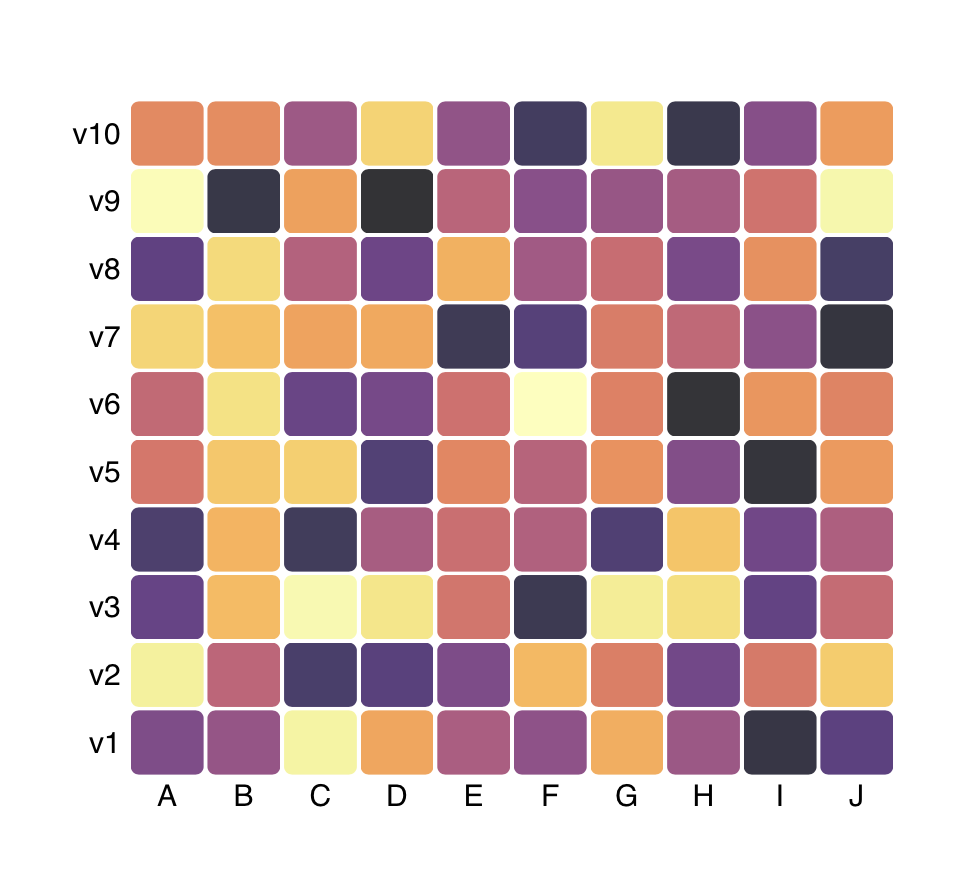
\includegraphics[width=0.4\textwidth]{doc/img/heatmap-without-meta.png}} 
    \subfigure[]{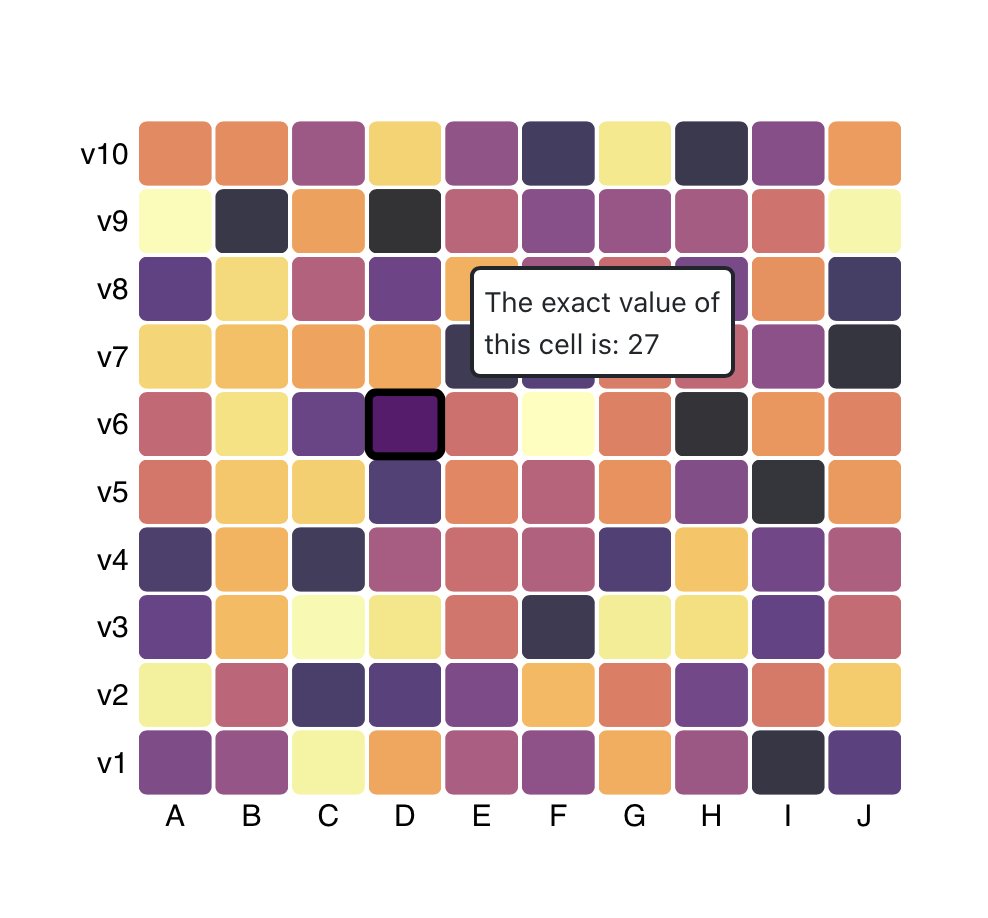
\includegraphics[width=0.4\textwidth]{doc/img/heatmap-with-meta.png}}
    \caption{(a) Heatmap without metadata (b) Heatmap with metadata}
    \label{fig:foobar}
\end{figure}

wollten eine cleane oberfläche, die interactive ist


%------------------------------------------------------------------------------------- (Introduction-ENDE)


WIP
similar systems you know


WIE
o Your project solution

WIP
Development environment
- language
- libraries
- ...

WIP
Implemented functionalities

stamming


WIE
experimitieren mit feates 
how to configure stamming
welche parameter haben wir gewählt

experimentierten mit 
sonetten und comedy, um unterschiede zu erkennen.
erkenntnis was, dass die einen charaktere mehr reden als andere
gab es outlier
gab es data preparation, wir haben die daten ausgegeglidert.


cluster-meta data wurde anfang implementiert, um schneller dinge interpretieren oder vergleichen zu können, wurde aber vom browser bei multipler dateiauswahl nur für eine datei ausgegeben

\begin{figure}
    \centering
    \subfigure[]{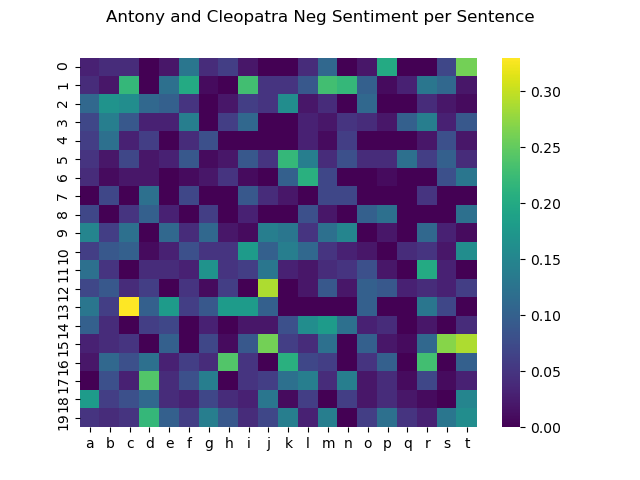
\includegraphics[width=0.24\textwidth]{img/Antony and Cleopatra Neg8.png}} 
    \subfigure[]{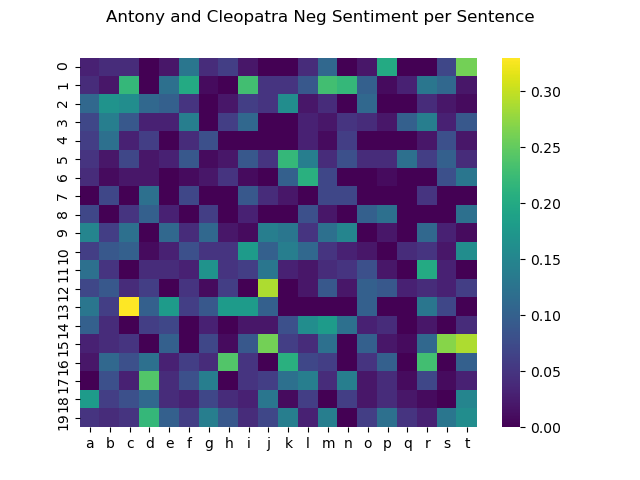
\includegraphics[width=0.24\textwidth]{img/Antony and Cleopatra Neg8.png}} 
    \subfigure[]{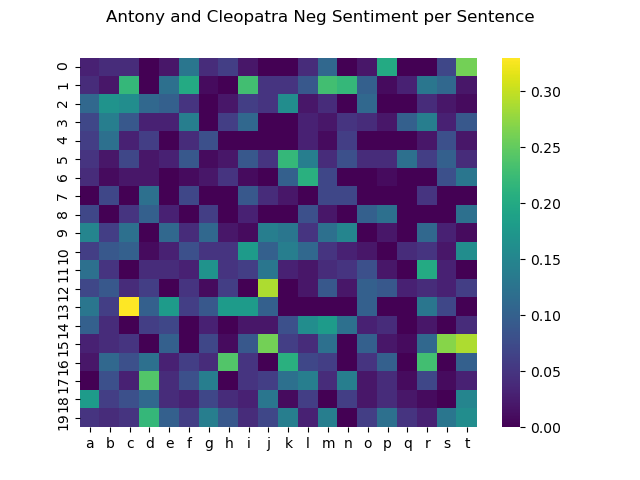
\includegraphics[width=0.24\textwidth]{img/Antony and Cleopatra Neg8.png}}
    \caption{(a) blah (b) blah (c) blah}
    \label{fig:foobar}
\end{figure}


WIP
Description of supported user operations (workflows)

WIE
Application demonstration
- Demonstrate the supported user operations by a walkthrough of a hypothetical
user Alice considering the used data

- Describe how and where searching and exploring are possible
- Describe interesting findings and observations you made when applying your solution to the data
- Discussion of advantages
- Discuss limitations and future developments to do
           



%------------------------------------------------------------------------------------- (References)
\section{References}
WIE

References Hints for the report:
- NOT more than 10 pages + appendix
- Make use of images/screenshots for your results

- Make use of diagrams to show system architcute or workflows


\begin{figure}
    \centering
    \subfigure[]{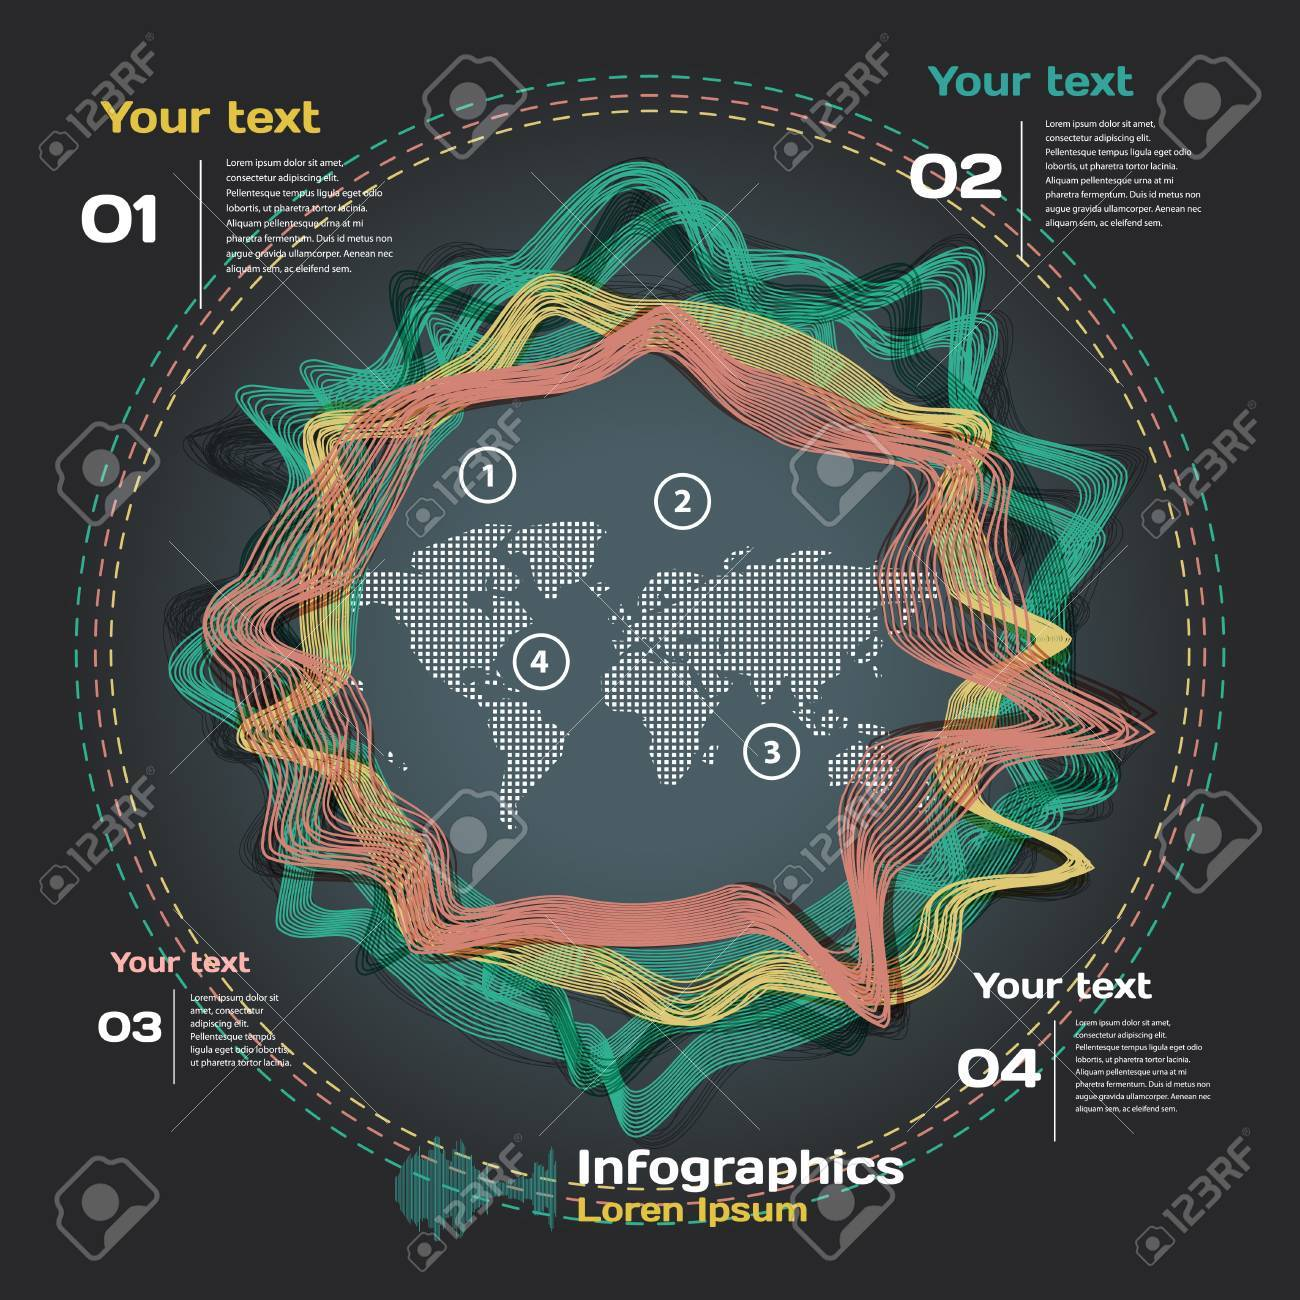
\includegraphics[width=0.5\textwidth]{doc/img/circular.jpg}} 
    \caption{Word frequency per Document \href{https://www.123rf.com/photo_36990141_stock-vector-infographics-with-sound-waves-on-world.html}{Copyright to Vladimir Arkatov}}
    \label{fig:circle-digram}
\end{figure}


\begin{figure}
    \centering
    \subfigure[]{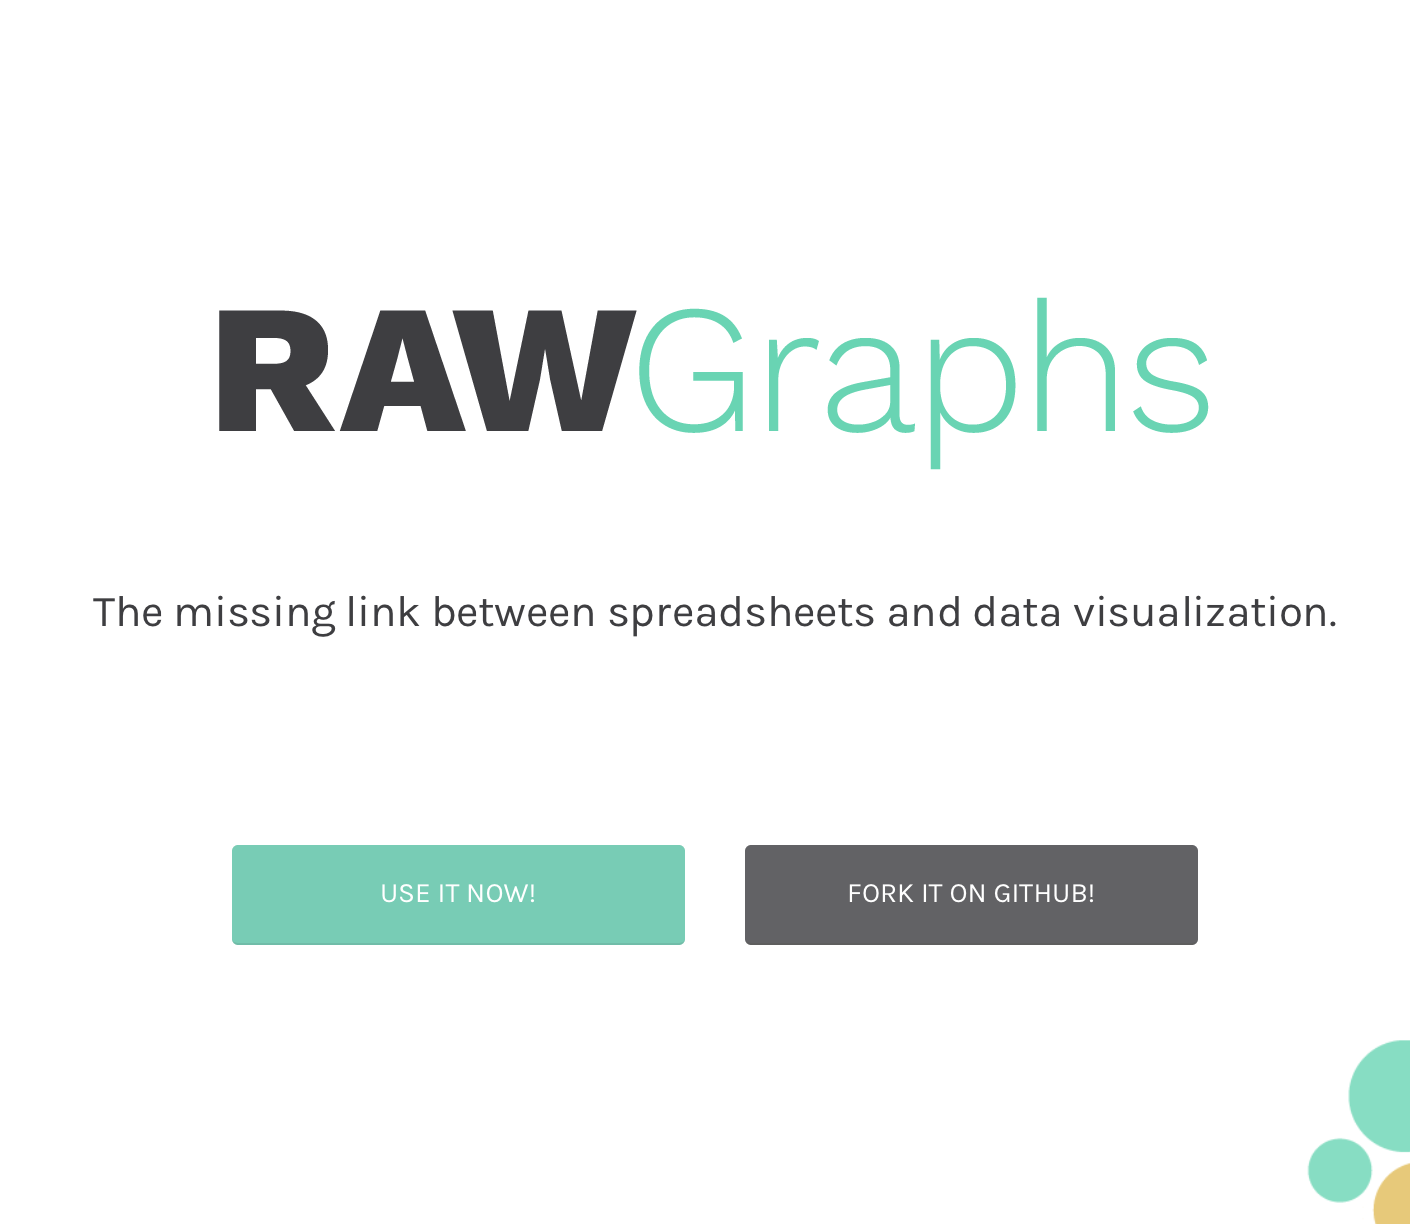
\includegraphics[width=0.5\textwidth]{doc/img/raw.png}} 
    \caption{\href{https://rawgraphs.io}{Designvorlage für Website}}
    \label{fig:website-reference}
\end{figure}





%------------------------------------------------------------------------------------- (Handling)
\newpage
\section{Handling}
WIP
user tasks to support

es gibt keine einschränkung bei der anzahl der dateien
limits 
es gibt lediglich ein limit beim zu verwendete

%------------------------------------------------------------------------------------- (Problems-ENDE)


%------------------------------------------------------------------------------------- (Problems)
\newpage
\section{Problems}
WIP
Search poblems
Exploration problem
WIE
\begin{itemize}
    \item[+] XXXXXXXXXXXX
    \item[-] YYYYYYYYYYYY
\end{itemize}


Probleme
Javascript biliotheken mit interaktiven heatmap 
heatmap mit hover effect for interactivity was only loaded each time for one file. 
that was the reason why we changed the plan and implemented it in such a way that the server creates heatmaps as images and creates a result page out of them.

multiple platformen, windows mac coused during programming problems becuase of path types

the browser cache was a BIG PROBLEM !!! Dieser leert sich nach dem versenden der Dateien an den Server und erfordert einen Neustart der GUI-oberfläche, da durch diesen Vorgang das benötigte Javascript file vom speicher geflashed wird.


mehr merhmacher dateiasuwahl muss derzeit noch zusätzlich die datei über der gewollten dateien ausgewählt werden. 


Calculating the position of points in a circle
https://stackoverflow.com/questions/5300938/calculating-the-position-of-points-in-a-circle

curveVertex
dabei werden die Punktkorrdinaten auf einem Kreis berechnet und danach einzeln mittels vertex kurve verbunden


%------------------------------------------------------------------------------------- (Problems-ENDE)







\newpage
%------------------------------------------------------------------------------------- (Development of our Tool)
\section{Development}
In this section we divide the three areas of software engineering that were developed in the creation of our tool. 

Implemented Featus


\subsection{Back-End: Feature Extraction}

Using NLP, we should be able to obtain features from a given text. Features such as word length, sentence length, sentiment of a sentence, etc\ldots We developed the file \texttt{feature\_extraction.py} to take care of just that. We used the programming language \texttt{Python} for this task due to it being incredibly powerful and easy to use in data-related tasks. Furthermore the \texttt{Natural Language Toolkit} library is supported by \texttt{Python}. This tool allows the programmer to use symbolic and statistical natural language processing for the English language.

\subsubsection{Natural Language Toolkit}

The \texttt{Natural Language Toolkit} (or NLTK) library is downloaded and installed into one's \texttt{Python} environment through the following line of code:

\begin{minted}{python}
nltk.download()
\end{minted}

From the NLTK library we use the following functions:
\begin{itemize}
    \item[--] Sentence Tokenizer: from a text, return a list of the entire text separated per sentence.
    \item[--] Word Tokenizer: from a text, return a list of the entire text separated per word.
    \item[--] Porter Stemmer: from a given word, return the root of it using a Porter Stemmer algorithm.
    \item[--] Stop Words: returns a list of all stop words from the English language (words with no inherent meaning - such as the words "the" and "a".)
    \item[--] Sentiment Intensity Analyser: from a sentence, return a dictionary containing the negative, neutral, positive, and compound values from that sentence.
\end{itemize}

We imported them into our \texttt{Python} file as such:

\begin{minted}{python}
from nltk.tokenize import sent_tokenize, word_tokenize, \
    TextTilingTokenizer
from nltk.stem import PorterStemmer
from nltk.corpus import stopwords
from nltk.sentiment.vader import SentimentIntensityAnalyzer
\end{minted}

Our \pythoninline{class FeatureExtractor} is defined as follows:
\begin{minted}{python}
class FeatureExtractor(object):
  exclude_stop_words =   True
  stem_words =     True
  filter_integers =   True
  exclude_duplicates =  True

  ps = None

  average_word_length_per_sentence =  None
  words_per_sentence =                None
  length_per_sentence =               None
  richness_per_sentence =             None
  richness_per_x_words =              None
  richness_per_sentence_stemmed =     None
  richness_per_x_words_stemmed =      None
  sentiment_per_sentence =            None
  digit_count_per_sentence =          None

  def __init__(self, exclude_stop_words = False, \
        stem_words = False,  filter_integers = False, 
        exclude_duplicates = False):
    self.exclude_stop_words = exclude_stop_words 
    self.stem_words = stem_words 
    self.filter_integers = filter_integers
    self.exclude_duplicates = exclude_duplicates

    self.ps = PorterStemmer()
\end{minted}
We will now elaborate on two method functions. One of them is able to extract features from the document, and the other is able to package the results into a format useful for heatmap creation.

\begin{python}
\input{src/file-1.py}
\end{minted}

In the code snippet above, we are trying to get the average word length every \texttt{x} amount of words. To do this, we must first tokenize the \texttt{parameter} using a tokenizer from the NLTK library. The variables \texttt{tokens} contains a list of all words in the text. We then iterate through the words. At every word, we increase our word counter variable \texttt{word\_count} by one and our word length counter \texttt{word\_len} by the size of the current word we are looking at. Notices that we are only looking at words that are not exclusively a punctuation. Once our \texttt{word\_count} counter reaches \texttt{x}, then we append the value of the \texttt{word\_len} variable divided by our \texttt{x} onto our \textit{result} list. We then reset our two counter variables. Once we have gone through all words, if there are words that we have not accounted for yet, we append them now. Finally, we return our \texttt{result} list. This list will contain the average length of words every \texttt{x} words. 

The other features follow a similar structure. If we want to get the average sentence length per \texttt{x} words, we would follow the snippet above but change the tokenizer method from using the word tokenizer to the sentence tokenizer. If we cared about getting the average sentence length of every length, we disregard the counters and the \texttt{x} variable, etc\ldots

The next step in our feature extraction script is to grab this resulting list and converting it into an $\texttt{n} \times \texttt{n}$ matrix. In our demo, we set our \texttt{n} to $20$. The way we did it can be seen in the snippet below.

\begin{python}
def chunkList(self, n, array):
  avg = len(array) / float(n * n)
  result = []
  row = []
  last = 0.0

  while last < len(array):
    tmp = array[int(last):int(last + avg)]
    row.append(0 if not tmp else (sum(tmp)/len(tmp), 2))
    if len(row) == n and (last + avg) < len(array):
      result.append(row)
      row = []
    last += avg
  if len(result) == 19:
    result.append(row)

  return result
\end{python}

The function \textit{chunkList} grabs a value for \texttt{n} and an array. We want to turn this list into a list of \texttt{n} lists each consisting of \texttt{n} amount of elements. To do this, it first compute the \texttt{avg} variable. This variable lets the algorithm how many elements of the array should be grouped together to end up with our required size. It divides the length of the array by $\texttt{n}^2$. The \texttt{while} loop iterates through the array initially grouping an \texttt{avg} amount of elements, grabbing the mean and appending it onto a \texttt{tmp} list. The \texttt{last} variable is added with \texttt{avg}. In the next iteration, the loop groups an \texttt{avg} amount of elements starting from the \textit{last} index. This is done \texttt{n} times. Once this occurs, the \texttt{tmp} list, which now contains \texttt{n} elements is added to the \texttt{result} variable. The \texttt{tmp} list is then reset. The loop continues until the \texttt{result} variable is of size $\texttt{n} \times \texttt{n}$ and the list is returned. 

This $\texttt{n} \times \texttt{n}$ list is fed to another script which is focused on creating a heatmap based off of the values in this list.
\subsection{Back-End: Server}

\subsection{Front-End}







\section{Further Development}

We started this project with the idea that we would be able to train this algorithm to be able to distinguish historic texts from non-historic text. The idea is that an algorithm, when fed all of these features and texts as training data would realize that the amount of digits a text has is a pretty important feature on historic text and not on any other literary genre. However, due to Shakespeare's style, this was quite troublesome. There are seldom any digits in his texts that could be found by a neural network or machine learning algorithm. The project was then put on ice. 

The idea, however, is not something that could be easily pivoted, given the right motivation and deadline. One could always create a neural network from these features to build a literature genre predictor. What could be interesting as well is to create an ensemble method such as Random Forests to, instead of trying to predict the genre of a text, try to learn which features are the most important to predict genre with. With our initial idea, we knew that digit count was quite important for historical text. As we were unable to create a neural network to predict genre, we might have been able to create some sort of machine learning algorithm (Random Forests) to find out what other feature might strongly correlate to historical data. 

Shakespeare's works, however, are quite rich in genre components within his texts. This makes using his works to develop such an algorithm incredibly difficult. Instead it would be best to use Shakespeare's texts as a validation dataset to really put an AI algorithm to the test. Sadly, this was out of the scope of our project. However, this finding might prove useful for anyone working on literature genre prediction.
%------------------------------------------------------------------------------------- (Contribution)
\newpage
\section{Contributions}
\begin{itemize}
  \item Richard Hohensinner \\ (design, coding, application, report writing)
  \item Inti Gabriel Mendoza Estrada \\ (design, coding, application, report writing)
  \item Jürgen Suntinger-Schrampf \\ (design, coding, application, report writing)
\end{itemize}
%------------------------------------------------------------------------------------- (Contribution-ENDE)






%\section{First Section}
%\subsection{A Subsection Sample}
%Please note that the first paragraph of a section or subsection is
%not indented. The first paragraph that follows a table, figure,
%equation etc. does not need an indent, either.
%
%Subsequent paragraphs, however, are indented.
%
%\subsubsection{Sample Heading (Third Level)} Only two levels of
%headings should be numbered. Lower level headings remain unnumbered;
%they are formatted as run-in headings.
%
%\paragraph{Sample Heading (Fourth Level)}
%The contribution should contain no more than four levels of
%headings. Table~\ref{tab1} gives a summary of all heading levels.
%
%\begin{table}
%\caption{Table captions should be placed above the
%tables.}\label{tab1}
%\begin{tabular}{|l|l|l|}
%\hline
%Heading level &  Example & Font size and style\\
%\hline
%Title (centered) &  {\Large\bfseries Lecture Notes} & 14 point, bold\\
%1st-level heading &  {\large\bfseries 1 Introduction} & 12 point, bold\\
%2nd-level heading & {\bfseries 2.1 Printing Area} & 10 point, bold\\
%3rd-level heading & {\bfseries Run-in Heading in Bold.} Text follows & 10 point, bold\\
%4th-level heading & {\itshape Lowest Level Heading.} Text follows & 10 point, italic\\
%\hline
%\end{tabular}
%\end{table}
%
%
%\noindent Displayed equations are centered and set on a separate
%line.
%\begin{equation}
%x + y = z
%\end{equation}
%Please try to avoid rasterized images for line-art diagrams and
%schemas. Whenever possible, use vector graphics instead (see
%Fig.~\ref{fig1}).
%
%\begin{figure}
%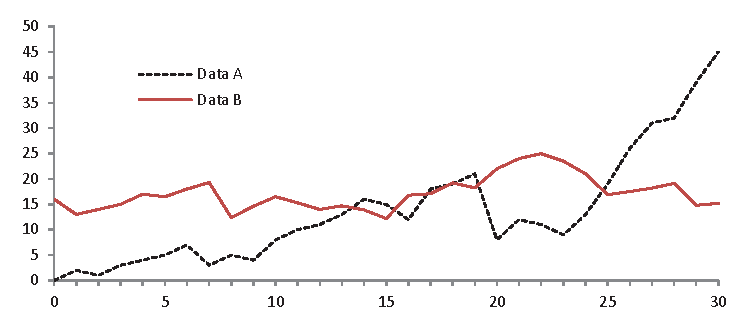
\includegraphics[width=\textwidth]{fig1.eps}
%\caption{A figure caption is always placed below the illustration.
%Please note that short captions are centered, while long ones are
%justified by the macro package automatically.} \label{fig1}
%\end{figure}
%
%\begin{theorem}
%This is a sample theorem. The run-in heading is set in bold, while
%the following text appears in italics. Definitions, lemmas,
%propositions, and corollaries are styled the same way.
%\end{theorem}
%%
%% the environments 'definition', 'lemma', 'proposition', 'corollary',
%% 'remark', and 'example' are defined in the LLNCS documentclass as well.
%%
%\begin{proof}
%Proofs, examples, and remarks have the initial word in italics,
%while the following text appears in normal font.
%\end{proof}
%For citations of references, we prefer the use of square brackets
%and consecutive numbers. Citations using labels or the author/year
%convention are also acceptable. The following bibliography provides
%a sample reference list with entries for journal
%articles~\cite{ref_article1}, an LNCS chapter~\cite{ref_lncs1}, a
%book~\cite{ref_book1}, proceedings without editors~\cite{ref_proc1},
%and a homepage~\cite{ref_url1}. Multiple citations are grouped
%\cite{ref_article1,ref_lncs1,ref_book1},
%\cite{ref_article1,ref_book1,ref_proc1,ref_url1}.
%%
%% ---- Bibliography ----
%%
%% BibTeX users should specify bibliography style 'splncs04'.
%% References will then be sorted and formatted in the correct style.
%%
%% \bibliographystyle{splncs04}
%% \bibliography{mybibliography}
%%
%\begin{thebibliography}{8}
%\bibitem{ref_article1}
%5Author, F.: Article title. Journal \textbf{2}(5), 99--110 (2016)
%
%\bibitem{ref_lncs1}
%Author, F., Author, S.: Title of a proceedings paper. In: Editor,
%F., Editor, S. (eds.) CONFERENCE 2016, LNCS, vol. 9999, pp. 1--13.
%Springer, Heidelberg (2016). \doi{10.10007/1234567890}
%
%\bibitem{ref_book1}
%Author, F., Author, S., Author, T.: Book title. 2nd edn. Publisher,
%Location (1999)
%
%\bibitem{ref_proc1}
%Author, A.-B.: Contribution title. In: 9th International Proceedings
%on Proceedings, pp. 1--2. Publisher, Location (2010)
%
%\bibitem{ref_url1}
%LNCS Homepage, \url{http://www.springer.com/lncs}. Last accessed 4
%Oct 2017
%\end{thebibliography}




\end{document}
%------------------------------------------------------------------------------------- (Dokument-ENDE)
